\documentclass{article}
\usepackage{graphicx} % Required for inserting images
\setlength\parindent{24pt}
\usepackage{geometry}
\usepackage{caption}
\usepackage{subcaption}
\usepackage{hyperref}
\renewcommand{\baselinestretch}{1.2}
\usepackage{pgfplots}
\usepackage{tikz}
\usepackage{array}
\usepackage{booktabs}
\pgfplotsset{compat=1.17}
\usepackage{amsmath}

\title{HW5}
\author{Delibas, Sabirenur\\
  \texttt{sabirenurd@gmail.com}
  \and
  Ulkutasir, Batuhan\\
  \texttt{ulkutasir.batuhan@gmail.com}}
\date{June 2024}
\geometry{left=2.5cm, right=2.5cm, top=2cm, bottom=2cm}
\begin{document}

\maketitle

\section{Introduction}
In this report, we will examine the parallelization and performance enhancement of computational algorithms using GPU computing with CUDA, which stands for Compute Unified Device Architecture. Throughout this course, our main focus was parallelization and optimizing Lloyd's k-means clustering algorithm. To achieve this ultimate goal, we have used many different computation methods based on CPU programming. From OpenMP to MPI we have learned multithreading, parallel operations, and distributing tasks across different cores. In these operations, CPU processors handling all the communications and controlling the sequence. On the other hand, Nvidia CUDA provides a more explicit and flexible approach to parallelism, by using the massive parallel processing capabilities of GPUs. Unlike general purpose CPUs, GPUs are specially designed to handle thousands of threads concurrently, by their simpler yet effective chip design. Ultimately increasing performance of parallelized tasks. Therefore, this study will compare performance of CUDA-based parallel algorithm across various data sets and configurations, and demonstrate the benefits. At the end of the report, the advantages of CUDA will be demonstrated, by comparing execution times and overall performance from the algorithms that built in HW2 and HW3.


\section{Implementation Details}
\textbf{Host and Device Operations:} To explain GPU computing first thing to explain is the difference of host and device separation. In GPU computing basically both of the GPU and CPU handles the operations. The term "host" refers to CPU and its associated memory and its operations. The host is responsible for running the main application code controlling the execution order of "kernel functions" and launching them when needed. It basically operates as the previous coding techniques that examined before.

On the other hand, the "device" refers to the GP, which is specially designed for high-speed parallel computations. Therefore in CUDA, GPU handles the computationally intensive parts of the application. These intensive parts generally launched (or called) by the host and refereed as "Kernel Functions". Separated from CPU, GPU has its own memory space, allocated by "cudaMalloc" commands. Thus it requires explicit data transfers commands as "cudaMemcpy" between the host and device, synchronized when needed. 


\textbf{Kernel Functions:} In CUDA, kernel functions are functions that run on the GPU. They are defined using the \_global\_ qualifier. Each kernel is executed by multiple threads in parallel. 

\texttt{distanceKernel}: This one calculates the Euclidean distances from each point to every centroid.

\texttt{assignPointsKernel}: Here, we assign each point to the nearest centroid based on the distances we calculated earlier.

\texttt{updateCentroidsKernel}: This kernel function updates the positions of the centroids based on the points assigned to them.

\texttt{normalizeCentroidsKernel}: Lastly, we have the normalizeCentroidsKernel. It takes care of normalizing the centroids by averaging the points assigned to each one.


\textbf{Thread Hierarchy:}  CUDA organizes threads into a hierarchy of grids and blocks. Each thread within a block has a unique thread ID. Threads within a block can cooperate by sharing data through shared memory and synchronizing their execution. 

\texttt{blockIdx.x}, \texttt{blockDim.x}, and \texttt{threadIdx.x} are used to determine the unique thread ID within the grid. This ID is used to index data and perform parallel computations.
We use a 1D grid of 1D blocks for simplicity, where the number of blocks is calculated as \[
\left(\frac{Np + \text{THREADS\_PER\_BLOCK} - 1}{\text{THREADS\_PER\_BLOCK}}\right)
\]

\textbf{Memory Management:} CUDA provides various types of memory for different purposes. Global memory is allocated using cudaMalloc and freed using cudaFree. Memory allocation and management are critical for efficient CUDA programming, ensuring that data is available to GPU threads during kernel execution. 

\textbf{Memory Transfer:} Data must be transferred between the host (CPU) and device (GPU) before and after kernel execution. cudaMemcpy is used for these transfers as explained before. Although these are essential execution codes over usage might cause delays and non-optimised results.

\textbf{Synchronization:} Synchronization ensures that all threads have completed their execution before the program proceeds. cudaDeviceSynchronize is used to synchronize the host with the device, ensuring that all preceding kernel executions and memory operations are completed.

\textbf{Execution Time Measurement:}
We measure the execution time with CUDA events. The start and end time of the execution of the kmeans algorithm is recorded using the \texttt{cudaEventRecord} function. The elapsed time is then calculated in by using \texttt{cudaEventElapsedTime} in order to be transformed in second to report.  


\section{Results \& Discussion}

\textbf{Elapsed Execution Times:}  This is the first section we would like to discuss in our code. We have compared the given datasets and their execution times in Table \ref{tab:data_details}. Naturally, an increasing time pattern by increasing the number of data points is evident. A very significant output is that the three-dimensional dataset converged immensely fast. This implies the significance of parallel operations powered by GPU computing. However, the elapsed time for the "Birch" dataset, containing 100,000 data points, was unexpectedly high at 25.6 seconds. This anomaly can be might be caused by our method of parallelization for the distance calculations, where the device computes distances between each pair of data points. At the level of this huge data cluster calculating distances was tedious process. This design selection ensured accurate centroid calculations by trading of from time

\begin{table}[h!]
    \centering
    \begin{tabular}{|>{\centering\arraybackslash}m{3cm}|>{\centering\arraybackslash}m{2cm}|>{\centering\arraybackslash}m{3cm}|>{\centering\arraybackslash}m{3cm}|}
        \hline
        \textbf{Data Set Name} & \textbf{Dimension} & \textbf{Number of Data Points} & \textbf{Elapsed Time (sec)} \\ \hline
        Hepta & 3D & 212 & 0.003 \\ \hline
        Smile & 2D & 1000 & 0.012 \\ \hline
        Circle & 2D & 4000 & 0.041 \\ \hline
        Isolation & 2D & 9000 & 0.057 \\ \hline
        Brich & 2D & 1000000 & 25.626 \\ \hline
    \end{tabular}
    \caption{Elapsed Time of Different Data Sets Compared in Seconds}
    \label{tab:data_details}
\end{table}


\textbf{Overall Logic and Structure Comparison:} Secondly, we have explored various parallelization methods for C programming so far. We must admit that implementing GPU computation for Lloyd's K-means algorithm was a challenging task. Additionally, using Google Colab  was also another challenge due to limited GPU times. However, when compared to MPI and its general operational syntax like rankings, shared threads, and buffered communications GPU programming becomes easier to comprehend. We believe that GPU employs a similar strategy as creating sub-functions. Thinking the host as the main function and the device operations as its sub-functions simplified our understanding since we found kernel functions easier to manage than shared multi-ranked threading operations. These approaches are also reflected in the number of lines written: the GPU parallelized code consists of 322 lines, while the MPI version has 260 lines, demonstrating that similar levels of parallelization could be achieved with fewer commands in different approaches.

\begin{figure}[htb]
    \centering
    \begin{subfigure}[b]{0.45\textwidth}
        \centering
        \includegraphics[width=\textwidth]{Isolation.PNG}
        \caption{Resulting centroid points of Isolation data set obtained by GPU computation}
        \label{fig:image3}
    \end{subfigure}
    \hfill
    \begin{subfigure}[b]{0.50\textwidth}
        \centering
        \includegraphics[width=\textwidth]{Circles.PNG}
        \caption{Resulting centroid points of Circles data set obtained by GPU computation}
        \label{fig:image4}
    \end{subfigure}
    \caption{Accuracy of the centroid locations for data sets named Isolation and Circles}
    \label{fig:sidebyside2}
\end{figure}

\textbf{Computation Time Differences with Serial and OpenMP Computation:}
Finally, this is consistently most important part of this report as we always examined importance of the parallelization in this course. As discussed in the elapsed time discussion we believe we have successfully implemented the GPU computation by delivering accurate centroid results in short time in almost of the data sets. As we did in HW 2 we wanted to demonstrate centroid locations for each clusters. They are given for two set of data in the Figure \ref{fig:sidebyside2}. It is also evident that our code has room for improvements as it operates poorly in the Brich dataset. Therefore it is not included in the computation time comparison as it would be tedious to demonstrate that much difference. In the Figure \ref{fig:timecomp} computation times for different number of data clusters compared in between three computing methods where Serial, OpenMP and GPU.

\begin{figure}[htb]
    \centering
    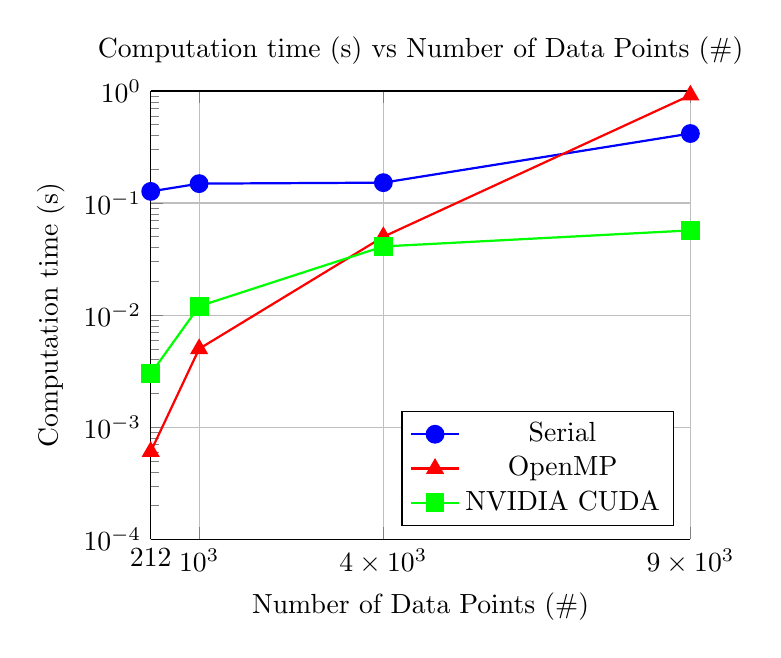
\begin{tikzpicture}
\centering
    \begin{axis}[
        title={Computation time (s) vs Number of Data Points (\#)},
        xlabel={Number of Data Points (\#)},
        ylabel={Computation time (s)},
        axis y line*=left,
        ymin=0.0001, ymax=1,
        xmin=212, xmax=9e3,
        ymode=log,
        xtick={212, 1e3, 4e3, 9e3},
        xticklabels={$212$,$10^3$,$4 \times 10^3$,$9 \times 10^3$},
        grid=major,
        legend entries={Serial, OpenMP, NVIDIA CUDA},
        legend pos= south east
    ]
    % First line
    \addplot[
        blue, 
        thick, 
        mark=*,
        mark options={scale=1.5}
    ] coordinates {
       (212, 0.127) (1e3, 0.149) (4e3, 0.152) (9e3, 0.417) 
    };
    
    % Second line
    \addplot[
        red, 
        thick, 
        mark=triangle*,
        mark options={scale=1.5}
    ] coordinates {
       (212, 0.0006053) (1e3, 0.005) (4e3, 0.05) (9e3, 0.916) 
    };
    
    % Third line
    \addplot[
        green, 
        thick, 
        mark=square*,
        mark options={scale=1.5}
    ] coordinates {
       (212, 0.003) (1e3, 0.012) (4e3, 0.041) (9e3, 0.057) 
    };

    \end{axis}
\end{tikzpicture}
    \caption{Comparison of computation times (in logarithmic scale) in different data sets with three different computation methods.}
    \label{fig:timecomp}
\end{figure}



\section{Conclusion}
In conclusion, this report demonstrates an algorithm application with GPU computing method which is named NVIDIA CUDA. Unlike previous methods involving CPU-based parallelization with OpenMP and MPI, CUDA utilizes the massive parallel processing power of GPUs to handle computationally intensive tasks more efficiently. The separation between the host (CPU) and device (GPU) ensures a flexible and powerful approach to parallel computation. Although we could not fully optimize parallel operations since our code operates poorly in Brich data set we believe we have fully implemented Lloyd's k-means clustering algorithm using CUDA. If we focus on the Isolation data set (Np=9000) we can observe both the OpenMP and Serial computations were not able to match the speed of the optimized CUDA implementation, especially when it came to dealing with the larger problems. The overall performance and execution time benefits of using NVIDIA CUDA for GPU computing are evident and promising. We believe that we have shown the potential of GPUs in speeding up parallel computation by this homework.

\end{document}
